\section{Introduction. Neutrinos as Fundamental Standard Model Particles}

The Standard Model can be summarized in a table like one at fig. \ref{fig:StandardModel}. It includes three charged leptons, three neutrinos and six quarks and their antiparticles which are split into three generations. In addition, it includes gauge bosons, Higgs boson and three fundamental interactions: electromagnetic, strong and weak. Charged particles, which include three leptons (electrons, muons and $\tau$-leptons), all quarks, W-bosons and their antiparticles can interact electromagnetically, through exchange of virtual photon. Quarks also posses additional quantum number which is called "color" and can also participate in strong couplings, through exchange of gluons. All those particles and also neutrinos can interact through weak interactions through charged current (CC), by exchanging W-boson, and through neutral current (NC), by exchanging Z-boson. The corresponding Feynman diagrams for the NC and CC are shown at fig. \ref{fig:NuScattering}\\

\begin{figure}
\caption{Fundamental particles and interactions. Three generations of fundamental particles and interaction mediators. Charged leptons and quarks are subjects to electromagnetic interactions (through photons). Quarks can also interact strongly (through gluons). All leptons and quarks can interact weakly (through $W^{\pm}$ and $Z^0$ bosons). All these and only these fundamental particles are discovered at the moment. Source of picture: \cite{ref_fig_StandardModel}}
\label{fig:StandardModel}
\centering 
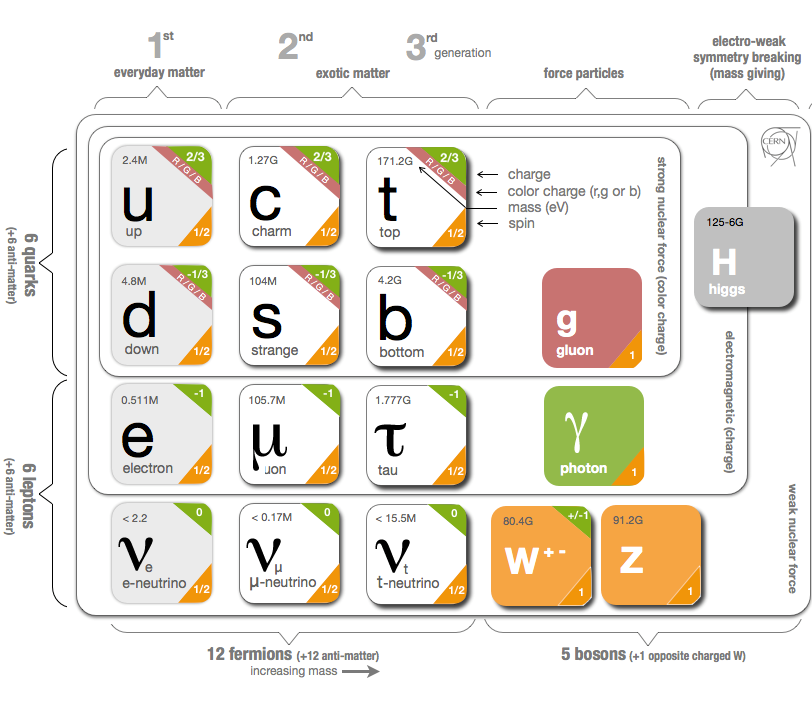
\includegraphics[width=0.83\textwidth, keepaspectratio=true]{figs/StandardModel.png}
\end{figure}

\begin{figure}
\caption{Feynman diagrams of neutral current (NC, left), and neutral current (CC, middle and right) neutrino scattering.}
\label{fig:NuScattering}
\centering
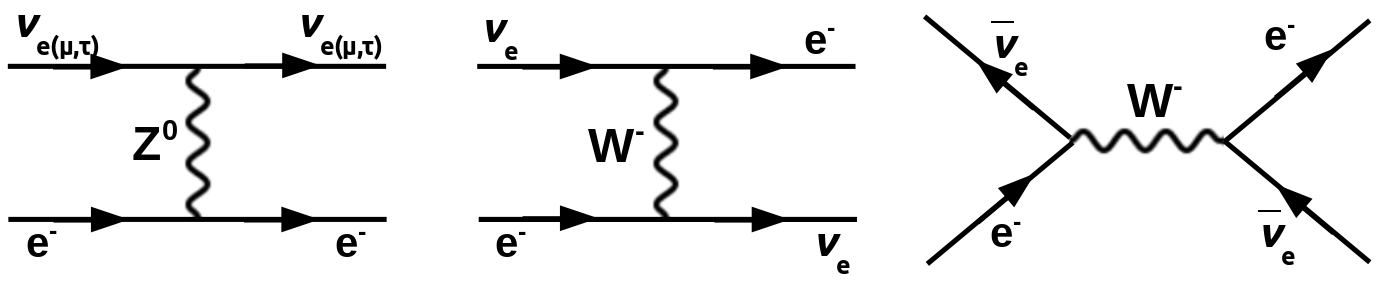
\includegraphics[width=0.80\textwidth, keepaspectratio=true]{figs/neutrinoScattering.png}
\end{figure}


All known substance in the Universe consists of millions of different molecules which are composed by hundreds different atoms. Each atom consists of certain number of protons, neutrons and electrons. All protons and neutrons are composed of three quarks (uud for proton and udd for neutron) which are glued together by strong interactions. Therefore, all known substance consists on only three fundamental particles from the fig. \ref{fig:StandardModel}: u- and d-quarks and electrons. Despite neutrinos are not part of substances, large number of them exists in the nature, without any human-built machines. Quoting \cite{ref_Griffiths}, 11.1: "John Bahcall, who was responsible for most of the calculations of solar neutrino abundances, liked to say that 100 billion neutrinos pass through your thumbnail every second; and yet they are so ethereal that you can look forward to only one or two neutrino-induced reaction in your body during your entire lifetime".\\
Two very common and well known interactions with neutrino participation are neutron beta decay and muon decay. The Feynman diagrams of these processes are shown at fig. \ref{fig:MuonAndNeutronDecays}. Mean lifetime of free neutron is $~15$ minutes and it decays as $n \rightarrow p + e^- + \bar{{\nu}_e} $ \cite{ref_PDG}. At the level of fundamental particles, neutron consists of two d-quarks and one u-quark and in the beta decay one of the d-quarks transfers to u-quark though the weak interaction mediated by $W^- $ boson. Thus, the proton, which consists of two u-quarks and one d-quark, is being produced. When this happens, the electron and electron antineutrino are emitted to preserve the charge and the lepton flavor number conserved. The examples of the neutron beta decay in nature include ${^{49}}{_{19}}K \rightarrow {^{40}}{_{20}}Ca$, ${^{64}}{_{29}}Cu \rightarrow {^{64}}{_{30}}Zn$, ${^3}{_1}H \rightarrow {^3}{_2}He$ \cite{ref_Griffiths} (the positive beta decay,  $p \rightarrow n + e^+ + {\nu}_e $, is forbidden for free proton by energy conservation law but it is allowed in certain cases when a proton is part of a nuclei). Such reactions are widely used for neutrino and antineutrino detection.\\
As for a muon, it's mean lifetime is $~2 {\mu}s$, and it decays as ${\mu}^- \rightarrow e^- + {\nu}_{\mu} + \bar{{\nu}_e}$ through the W boson. This process is also common in nature, in cosmic rays: muons are produced in the upper layers of the Earth atmosphere from the interaction of the particles coming from cosmic rays with the atmosphere molecules, for instance, as $p+p \rightarrow n+p+\pi^+$ with further pion decay $\pi^+ \rightarrow \mu^+ + \nu_\mu$ and then some number of muons decay $\mu^+ \rightarrow e^+ + \nu_e + \bar{\nu_\mu}$ while traveling through the atmosphere to the ground. The scheme of the shower in the Earth atmosphere induced by the primary incident proton is shown on fig. \ref{fig:cosmicMuons}.   

\begin{figure}
\caption{Feynman diagrams of (left) neutron and (right) muon decays. Neutron beta decay (d-quark of transfers to u-quark through the W-boson with emission of electron and antineutrino). Muon decay (muon decays to electron, neutrino and antineutrino through W-boson}
\label{fig:MuonAndNeutronDecays}
\centering
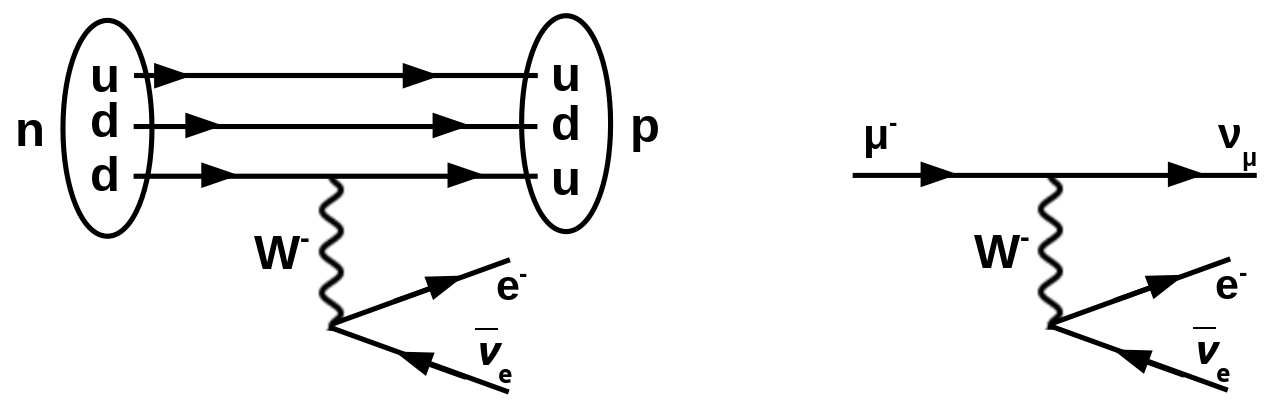
\includegraphics[width=0.70\textwidth, keepaspectratio=true]{figs/NeutronAndMuonDecays.png}
\end{figure}

\begin{figure}
\caption{Cosmic shower induced by scattering of the incident cosmic proton of an air molecule. Charged and neutron pions are born in the reaction and then they further decay as $\pi^0 \rightarrow \gamma\gamma$, $\pi^+ \rightarrow \mu^+ + \nu_\mu$, $\pi^- \rightarrow \mu^- + \bar{\nu_\mu}$.}
\label{fig:cosmicMuons}
\centering
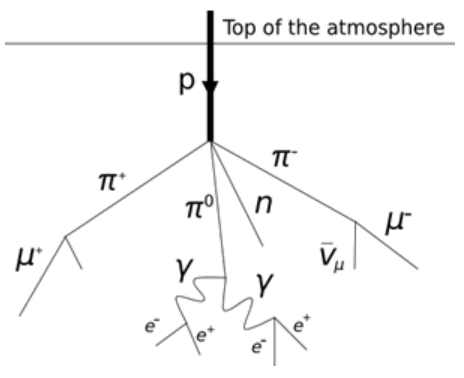
\includegraphics[width=0.60\textwidth, keepaspectratio=true]{figs/cosmicMuons.png}
\end{figure}



There are three flavors of neutrino, one for each generation: electron neutrino, muon neutrino, $\tau$-neutrino. And in the processes described above (neutron beta decay and muon decay) the lepton flavor numbers $L_e$, $L_{\mu}$ and $L_{\tau}$ are conserved. The table \ref{tab:LeptonFlavorNumber} shows the value of this number for all leptons and anti leptons. 

\begin{table}[h]
  \begin{center}
  \caption{ Lepton Flavor Number}
  \begin{tabular}{|c|c|c|c|}
     particles & $L_e$ & $L_{\mu}$ & $L_{\tau}$ \\ \hline
     $e^-,\nu_e$ &  +1  &  0  &  0  \\ \hline 
     $e^+, \bar{\nu_e}$ &  -1  &  0  &  0  \\ \hline 
     $\mu^-,\nu_{\mu}$ &  0  &  +1  &  0  \\ \hline 
     $\mu^+, \bar{\nu_{\mu}}$ &  0  &  -1  &  0  \\ \hline 
     $\tau^-,\nu_{\tau}$ &  0  &  0  &  +1  \\ \hline 
     $\tau^+, \bar{\nu_{\tau}}$ &  0  &  0  &  -1  \\ \hline 
  \end{tabular}
  \label{tab:LeptonFlavorNumber}
  \end{center}
\end{table}

The lepton flavor numbers are conserved in almost all particle physics processes and the only violation of this law observed by this time is the neutrino oscillations - the ability of neutrino to change flavor.\\ 
Chapter 2 of this paper reviews the theoretical background of the neutrino oscillations starting from simplified two-neutrinos model in vacuum to three-neutrinos model in presence of matter and also discussed possible mechanisms of neutrinos to get masses. Chapter 3 gives historical background to related experimental measurements including the first evidences of neutrino oscillations, milestones achieved by scientific community in measuring different neutrino oscillation parameters and the most recent experimental results. Chapter 4 explains need of the new experiment and gives overview of the proposed LB NF/DUNE experiment in terms of its physics program and experimental setup, it also discusses the advantages of the LBNF/DUNE comparing to the other experiments of this kind. Chapter 5 draws conclusions.  


